La interfaz de lectura ASD (Amplificator-Shaper-Discriminator)\cite{1999ATLASICs} es un sistema de 16 canales utilizado para la lectura de detectores TGC en la Big Wheel del experimento ATLAS, como se mencionó en la Sección \ref{sec:atlas}. El propósito principal de esta interfaz es detectar pulsos de alta frecuencia provenientes de detectores TGC, los cuales forman parte del Level-1 Trigger en el espectrómetro de muones. Cada canal se corresponde con un \textit{strip} o cable de un detector, por lo que al analizar las señales de salida de esta tarjeta permite determinar los vértices de interacción de muones con el detector.

La Figura \ref{img:asd-board} corresponde a una fotografía de esta interfaz, destacando sus conectores principales y sus canales de entrada. Los canales son llamados \textit{Hits} y se enumeran del 0 al 15. La interfaz ASD posee un conector de 40 pines para la conexión de su fuente de voltaje, transmisión de las señales de salida  e ingreso de pulsos de prueba. El detalle de cada pin se ilustra en la Tabla \ref{tab:asd-ports}, donde las columnas izquierdas corresponden a los terminales positivos de los pares diferenciales, mientras que las columnas derechas indican los terminales negativos.  %\sgcnote{y el punto? Mejorar la resolucion de la figura. Es una tabla. Seria mejor hacerla directo en latex.  En general, se nota que aca escribiste a la rapida sin revisar, y se nota una diferencia entre este texto y el resto (como pegado con chicle.  Debes evitar que eso se refleje en el documento.}

\begin{figure}[h]
	\centering
	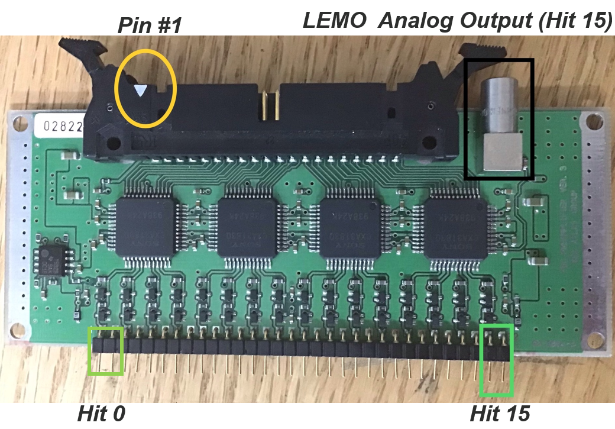
\includegraphics[scale=0.55]{asd-board.png}
	\caption{Interfaz de lectura ASD. Se destacan en la imagen sus canales (hit) del 0 al 15, su salida analógica LEMO y el primer pin en su conector de 40 posiciones.}
	\label{img:asd-board}
\end{figure}

% Please add the following required packages to your document preamble:
% \usepackage{booktabs}
\begin{table}[]
	\centering
	\caption{Detalle de los puertos en el conector de 40 posiciones en la interfaz ASD.}
	\begin{tabular}{@{}llll@{}}
		\toprule
		\textbf{Pin} & \textbf{Nombre} & \textbf{Nombre}                & \textbf{Pin} \\ \midrule
		1            & GND             & V$_{th}$                       & 2            \\
		3            & -3,0V           & GND                            & 4            \\
		5            & +3,0V           & +3,0V                          & 6            \\
		7            & test pulse      & $\overline{\mbox{test pulse}}$ & 8            \\
		9            & hit 0           & $\overline{\mbox{hit 0}}$      & 10           \\
		11           & hit 1           & $\overline{\mbox{hit 1}}$      & 12           \\
		13           & hit 2           & $\overline{\mbox{hit 2}}$      & 14           \\
		15           & hit 3           & $\overline{\mbox{hit 3}}$      & 16           \\
		17           & hit 4           & $\overline{\mbox{hit 4}}$      & 18           \\
		19           & hit 5           & $\overline{\mbox{hit 5}}$      & 20           \\
		21           & hit 6           & $\overline{\mbox{hit 6}}$      & 22           \\
		23           & hit 7           & $\overline{\mbox{hit 7}}$      & 24           \\
		25           & hit 8           & $\overline{\mbox{hit 8}}$      & 26           \\
		27           & hit 9           & $\overline{\mbox{hit 9}}$      & 28           \\
		29           & hit 10          & $\overline{\mbox{hit 10}}$     & 30           \\
		31           & hit 11          & $\overline{\mbox{hit 11}}$     & 32           \\
		33           & hit 12          & $\overline{\mbox{hit 12}}$     & 34           \\
		35           & hit 13          & $\overline{\mbox{hit 13}}$     & 36           \\
		37           & hit 14          & $\overline{\mbox{hit 14}}$     & 38           \\
		39           & hit 15          & $\overline{\mbox{hit 15}}$     & 40           \\ \bottomrule
	\end{tabular}
	\label{tab:asd-ports}
\end{table}

Como su acrónimo lo indica, la interfaz ASD (Amplificator-Shaper-Discriminator) amplifica la carga eléctrica captada desde un canal de un detector, modifica la forma del pulso eléctrico en cuanto a su tiempo de duración y a su amplitud de corriente con el fin de simplificar su posterior medición, y discrimina la amplitud del pulso mediante un circuito comparador. Esta comparación se realiza respecto a un nivel de voltaje ajustable para así descartar eventos de energía que estén por debajo el umbral de interés, y también para generar una señal de salida digital LVDS (Low-Voltage Differential signal)\cite{1996IEEESociety} cuya duración sea proporcional a la amplitud de pulso que ha estado por sobre el umbral de voltaje configurado. Esta técnica se conoce como TOT (Time-Over-Threshold) y es la mísma técnica utilizada en el detector LabPet II descrito en la sección \ref{par:labpet}.  En la Figura \ref{fig:sistema-completo}, este pulso digital se representa como el pulso digital rojo entre la interfaz de lectura y el sistema de adquisición de datos.
        
La interfaz ASD será utilizada conectándola a los \textit{strips} de los detectores sTGC fabricados para sTGC Minería. Dado que la interfaz posee 16 canales de entrada, es posible conectar los 16 canales de detección proveniente de un mismo detector prototipo sTGC. Así, con un solo detector y una interfaz es posible determinar vértices de interacción en un área de 225cm$^2$. Para un futuro escalamiento, utilizando dos detectores superpuestos y sus respectivas interfaces es posible determinar la trayectoria de los muones detectados. Además, analizar la duración de cada pulso emitido por las interfaces permite estimar la amplitud de la carga eléctrica depositada por el muon en el detector excitado.


\subsection{Circuito interno de Amplificación, Acondicionamiento y Discriminación}
La interfaz de lectura ASD tiene 16 canales que reciben impulsos de carga eléctrica provenientes de \textit{strips} o cables de detectores TGC, y emite señales digitales representando estos pulsos en formato LVDS según la norma IEEE LVDS Standard 1596.3-1996\cite{1996IEEESociety}.

Esta interfaz requiere una fuente de voltaje de $\pm$3V\cite{1999ATLASICs}, es capaz de recibir pulsos entre -1.2pC a +2.0pC sin saturarse y posee una frecuencia de entrada especificada de hasta 100KHz. La interfaz cuenta con un una entrada para pulsos de pruebas y una señal analógica de monitoreo proveniente de la etapa de preamplificación del canal 15, implementada con un conector LEMO.

En la Figura \ref{img:asd-circuit} se ilustra el circuito principal incluido en cada canal de la interfaz ASD. Cada canal tiene su propio preamplificador, un amplificador principal y un comparador\cite{1999ATLASICs}, donde la etapa de preamplificación tiene una ganancia de 0.8V/pC y el amplificador principal tiene una ganancia de 7 veces la señal entrante. La etapa de comparación compara la señal con un nivel de voltaje externo llamado \textit{V$_{th}$}. Si el pulso entrante tiene una amplitud de voltaje superior a $\frac{V_{th}}{2}$, el comparador emite una señal LVDS con una duración equivalente al tiempo durante el cual la amplitud del pulso entrante se mantuvo por sobre $\frac{V_{th}}{2}$. V$_{th}$ puede configurarse en un rango desde -0.5V a +0.5V, resultando en un umbral real de -0.25V a +0.25V en el comparador\cite{1999ATLASICs}. Así, es capaz de emitir señales digitales con duraciones entre 25ns y 45ns para pulsos de entrada con cargas entre 0.1pC y 0.5pC respectivamente.

Las señales digitales LVDS emitidas por las etapas de comparación incluidas en la interfaz ASD corresponden a las señales a ser muestreadas por el sistema de adquisición a diseñar en esta memoria de titulación. En el Capítulo \ref{cap:sadq} se define el sistema de adquisición en base a la cantidad, formato y duración de estas señales digitales.

\begin{figure}[h]
	\centering
	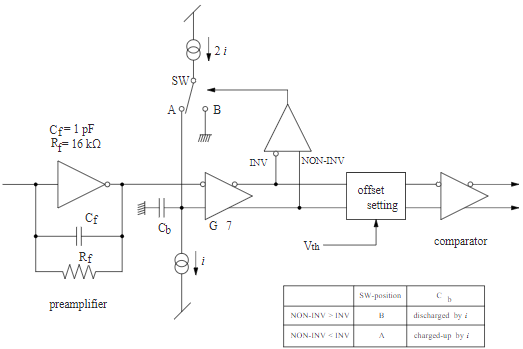
\includegraphics[scale=0.4]{asd-circuit.png}
	\caption{Diagrama de bloques del circuito principal para un canal de la interfaz ASD. Se indican la etapa de preamplificación, el amplificador principal de ganancia 7, y el comparador.}
	\label{img:asd-circuit}
\end{figure}

\sgcnote{y esto es relevante? afecta el funcionamiento?  Falta tambien una frase de cierre que concluya y conecte con la siguientes seccion.}
\sjgnote{Pensandolo bien yo diria que no es relevante este ejemplo y la diferencia entre valor esperado y medido no afecta al funcionamiento, porque se debe principalmente a que fue medido con los cables y herramientas incorrectos. Comente esta subseccion para quitarlo del escrito.}


